\documentclass[conference]{IEEEtran}
\IEEEoverridecommandlockouts

\usepackage{amsmath,amssymb}
\usepackage{booktabs}
\usepackage{graphicx}
\usepackage{array}
\usepackage{url}
\usepackage{algorithm}
\usepackage{algpseudocode}

\graphicspath{{figs/}}

\newcommand{\psic}{\psi}
\newcommand{\tstar}{t^{\ast}}

\begin{document}

\title{Support-Constrained Interpretable Subgroup Discovery for Survival
Outcomes: A Measured Operating Range}

\author{
\IEEEauthorblockN{Author Name}
\IEEEauthorblockA{Department of Computer Science\\
Amrita Vishwa Vidyapeetham\\
Kollam, India\\
email@example.com}
}

\maketitle

\begin{abstract}
Interpretable subgroup analyses are usually justified by the claim that they
identify patients who benefit more than the average. We test that claim for
CISCaRL, a support-constrained interpretable survival rule model, against the
simplest competitor, a constant model that assigns every patient the marginal
average treatment effect (ATE), for the fixed-time survival contrast
$\tau(730\mid x)=P(T^{1}>730\mid x)-P(T^{0}>730\mid x)$. Estimation is doubly
robust: per-arm Cox nuisances are cross-fitted, censoring is adjusted by a
conditional Cox model with a weight cap, and subgroup effects use augmented
inverse-probability-weighted (AIPW) influence functions. Discovery fits a
depth-3 CART to the AIPW pseudo-outcome; the selected leaf must contain at
least 200 discovery patients; its effect is re-estimated on a disjoint
validation partition; and treatment is recommended only if the validation
lower confidence bound exceeds zero. Discovery, validation and assessment are
disjoint (4000/2000/2000 at $n=8000$). At $n=2000$ no discovered rule model
beats the constant; from $n\approx6000$ the pseudo-outcome model does
($21.7\%$ lower held-out mean absolute error), and the frozen pipeline reaches
$19.9\%$ at $n=8000$. The support constraint raises coverage of the true region
from 0.23 to 0.51 at purity $0.82$ in a single-region design, and captured
benefit from 0.15 to 0.36 with two regions, with a $0\%$ null-benefit
treatment rate and decision efficiency $0.82$--$0.88$. A two-leaf extension captures more benefit but dilutes purity
from 0.86 to 0.70. Against a survival causal rule ensemble (SCRE) on identical
splits the frozen model is $0.003$--$0.006$ worse on patient-level mean absolute
error; a post-hoc empirical-Bayes shrinkage of leaf effects, confirmed on fresh
seeds, removes that deficit ($+0.0011$, $p=0.48$ with one region; $+0.0004$,
$p=0.76$ with two) without changing a single treatment decision. The model is
substantially purer ($0.89$ versus $0.44$--$0.60$) and about twice as beneficial
per treated patient. On ACTG175 the support constraint cannot be met at that sample size:
the model falls back to a 62-patient leaf and correctly abstains. The method is
a defensible point on the capture--purity frontier with a measured operating
range, not a universal improvement over the marginal ATE.
\end{abstract}

\begin{IEEEkeywords}
survival analysis, heterogeneous treatment effects, subgroup discovery, doubly
robust estimation, interpretable rules, abstention, AIPW.
\end{IEEEkeywords}

\section{Introduction}

Randomized controlled trials establish an average treatment effect, but
clinicians treat individuals. A subgroup analysis promises to convert the
average into a decision: who should be treated, how much benefit to expect, and
when the evidence is too weak to act. The promise is easy to state and hard to
verify, because it bundles three different requirements. Detection asks whether
treatment effects vary at all. Recovery asks whether the boundary between
benefiting and non-benefiting patients can be identified from a finite sample.
Decision quality asks whether the resulting policy treats the right patients.
A method can succeed at one and fail at another, and the failure is invisible
if only a single metric is reported.

Two failure modes dominate the applied literature. The first is the
\emph{constant baseline}: a subgroup model is presented without comparison to
the marginal ATE applied to everyone, so a method that simply reproduces the
average effect looks like a success. The second is \emph{selection optimism}:
the best leaf of a fitted tree is reported with an in-sample effect, which
overstates both its benefit and its precision. Both are avoidable, and avoiding
them changes what can be claimed.

This paper studies a deliberately simple competitor throughout: a constant
model that assigns every patient the marginal ATE estimated on training data.
If a subgroup model cannot beat that constant on held-out patients, its rules
add variance rather than information. An oracle that knows true region
membership but estimates its effect from the same data provides an upper bound
on what the design can deliver.

We call the method CISCaRL. Its frozen configuration, used for every result in
this paper, is C200. The number 200 is the minimum number of discovery patients
a candidate leaf must contain; it is not a count of trees, iterations or
features. C200 is therefore one configuration of one model, not a second model,
and the tables use the short label only for brevity.

Our contributions are five.
(i)~An honest evaluation design in which discovery, validation and assessment
are disjoint: rules and thresholds are fitted on discovery, leaf effects and
commitment on validation, and assessment is used only to score the frozen
model.
(ii)~A support-constrained selection rule that requires at least 200 discovery
patients in the high-benefit leaf, targeting the winner's curse that selects
small extreme leaves.
(iii)~A validation-based commitment layer that recommends treatment only when
the validation lower confidence bound exceeds zero, and otherwise abstains.
(iv)~A measured operating range and a reproducibility boundary, including the
sample size below which the rule model is worse than the constant.
(v)~Documented negative results for restricted mean survival time, support
tuning, random-forest stability selection, target blending, a two-leaf list and
a flexible-learner distillation, together with a head-to-head comparison
against a survival rule-ensemble method on identical splits.

We do not claim universal superiority, full recovery of the true region, or
unconditional robustness. The central empirical result is a boundary, and the
comparison against the rule ensemble is included precisely because it does not
favour our method on accuracy.

\section{Related Work}

Doubly robust estimation combines an outcome model with a treatment or
censoring model so that the contrast remains consistent if either is correct
\cite{bang}. Cross-fitting removes the overfitting bias of nuisance estimation
and underlies double/debiased machine learning \cite{dml}. AIPW
pseudo-outcomes provide patient-level signals whose conditional mean is the
treatment effect, and they are the building block of DR- and R-learner
approaches to heterogeneous effects \cite{drlearner,nie}. Meta-learners
organize the same idea around T-, S- and X-learner architectures
\cite{kunzel}.

For survival outcomes, causal survival forests estimate conditional effects
under right censoring using local estimating equations and orthogonal scores
\cite{csf}, while forest-based inference for heterogeneous effects is
established in the non-survival setting \cite{wager}. Tree-based subgroup
identification has a long history in clinical trials, from interaction-tree
search \cite{foster} to model-based recursive partitioning and its tutorial
literature \cite{lipkovich}. Rule ensembles occupy a complementary point: they
are interpretable by construction and flexible enough to approximate
nonlinearity \cite{rulefit}, and a survival extension has recently been
proposed as a causal rule ensemble \cite{scre}.

Stability selection \cite{stability} and constrained policy learning
\cite{policy} are established separately and inform the design used here: the
former motivates measuring reproducibility by refitting the whole procedure,
the latter motivates treating the subgroup as a policy with a coverage cost.
What is missing across these strands is a joint evaluation of discovery,
commitment and cost on the same splits. This work is not a new learner; its
contribution is the integration and evaluation of cross-fitted
censoring-adjusted estimation, support-constrained selection, validation-based
commitment, and an honest assessment of capture, purity, stability and decision
quality, including the sample-size boundary.

\section{Method}

\subsection{Notation and Estimand}

Let $T^{a}$ be the potential event time under treatment $a\in\{0,1\}$, $C$ the
censoring time, $T=\min(T^{a},C)$ the observed time, $\Delta=\mathbf{1}\{T^{a}\le
C\}$ the event indicator, $A\in\{0,1\}$ the treatment, and $X\in\mathbb{R}^{p}$
the baseline covariates. Treatment is randomized, so the propensity is
$e=P(A=1)=0.5$ and no propensity model is fitted. The conditional survival
function and the estimand are
\begin{align}
S_{a}(\tstar\mid x) &= P(T^{a}>\tstar\mid X=x),\label{eq:S}\\
\tau(\tstar\mid x) &= S_{1}(\tstar\mid x)-S_{0}(\tstar\mid x),\label{eq:tau}
\end{align}
with $\tstar=730$ days. The event is a composite of a CD4 decline of at least
50 cells, AIDS progression, or death, evaluated under the observed follow-up
process. Equation~\eqref{eq:tau} is a survival-probability contrast, not a
hazard ratio and not an intention-to-treat effect. For a subgroup defined by a
rule $r:\mathbb{R}^{p}\to\{0,1\}$ we write
\begin{equation}
\tau(r)=E\big[\tau(\tstar\mid X)\mid r(X)=1\big].\label{eq:taur}
\end{equation}

\subsection{Nuisance Estimation and AIPW}

Both nuisances are Cox models. For each arm, a Cox model is fitted on the
discovery partition and the baseline survival is evaluated at $\tstar$, giving
$\hat\mu_{a}(\tstar,x)=\hat S_{a}(\tstar\mid x)$. The censoring distribution is
estimated by a Cox model on $X$ and evaluated at $\tstar$, giving
$\hat G(\tstar\mid x)$. Nuisances are cross-fitted over five folds so that every
discovery patient is scored by models that did not use that patient.

With $e=0.5$, the inverse-probability-weighted outcome and the pseudo-outcome
are
\begin{align}
Y_{i} &= \frac{\mathbf{1}\{T_{i}>\tstar\}}{\hat G(\tstar\mid X_{i})},\\
\psi_{i} &= \frac{A_{i}-e}{e(1-e)}\big(Y_{i}-\hat\mu_{A_{i}}(\tstar,X_{i})\big)
+\hat\mu_{1}(\tstar,X_{i})-\hat\mu_{0}(\tstar,X_{i}),\label{eq:psi}
\end{align}
so that $E[\psi\mid X=x]=\tau(\tstar\mid x)$ when either nuisance is correct.
Weights are capped at $c=\min(Q_{0.99},20)$ per fold, computed from the fitting
rows only. Capping changes the estimand when it binds, so the capped weight
fraction and the effective sample size are reported rather than assumed
negligible.

\subsection{Pseudo-Outcome Tree Discovery}

A regression tree of depth three is fitted to $\psi$ on the discovery
partition with a minimum of 60 patients per leaf. Each leaf defines a candidate
rule $r_{k}$ as the conjunction of its split conditions, and leaf $k$ carries a
support $n_{k}$ and a discovery mean $\bar\psi_{k}$. Depth three keeps the
rules readable (at most three conditions) and the number of candidates small
(five to eight leaves in the designs studied).

\subsection{Support-Constrained Selection}

Maximizing $\bar\psi_{k}$ alone selects small extreme leaves, whose estimates
are dominated by noise. The selected leaf is therefore
\begin{equation}
k^{\star}=\arg\max_{k}\{\bar\psi_{k}: n_{k}\ge m\},\qquad m=200,
\label{eq:select}
\end{equation}
with the unconstrained argmax used, and explicitly flagged as a fallback, when
no leaf reaches $m$. The threshold is not tuned per dataset; it is frozen at
200 patients, roughly a tenth of the discovery partition in the main design.

\subsection{Validation-Based Commitment}

Discovery ranks leaves; it does not license a treatment recommendation. The
effect of the selected rule is re-estimated on the validation partition with
the AIPW estimator of Section~III-B using discovery-fitted nuisances:
\begin{equation}
\hat\tau(r_{k^{\star}})=\frac{1}{n_{\mathcal{V}}}\sum_{i\in\mathcal{V}}
\big(\hat\phi_{i}^{1}-\hat\phi_{i}^{0}\big) r_{k^{\star}}(X_{i}),
\label{eq:val}
\end{equation}
where $\hat\phi_{i}^{a}=\hat\mu_{a}+\mathbf{1}\{A_{i}=a\}/e\,(Y_{i}-\hat\mu_{a})$.
The standard error is the influence-function form
$\mathrm{SE}=\{n_{\mathcal{V}}^{-1}\sum_{i}(\hat\phi_{i}-\hat\tau)^{2}\}^{1/2}$
restricted to rule members, and the one-sided lower bound is
\begin{equation}
L=\hat\tau(r_{k^{\star}})-1.645\,\mathrm{SE}.
\label{eq:lcb}
\end{equation}
The model commits when $L>0$. Reporting is three-valued: \textsc{treat} if
$L>0$, \textsc{avoid} if the upper bound is below zero, and
\textsc{insufficient} otherwise, in which case no treatment is recommended and
predictions fall back to the marginal ATE. Because the interval conditions on
the rule selected on discovery, empirical coverage is approximately $93\%$
rather than $95\%$; this is stated wherever an interval is reported.
Algorithm~\ref{alg:c200} summarizes the frozen procedure.

\begin{algorithm}[t]
\caption{The frozen CISCaRL-C200 procedure}
\label{alg:c200}
\begin{algorithmic}[1]
\Require discovery $\mathcal{D}$, validation $\mathcal{V}$, assessment
$\mathcal{A}$; horizon $\tstar=730$; support floor $m=200$
\State cross-fit per-arm Cox outcome models and the censoring Cox over 5 folds
of $\mathcal{D}$
\State cap censoring weights at $\min(Q_{0.99},20)$ per fold
\State compute $\psi_{i}$ for $i\in\mathcal{D}$ with $e=0.5$
\State grow a depth-3 CART on $\psi$, \texttt{min\_samples\_leaf}${}=60$
\State extract leaves $r_{1},\dots,r_{K}$ with support $n_{k}$ and mean
$\bar\psi_{k}$
\If{$\exists k:n_{k}\ge m$}
  \State $k^{\star}\gets\arg\max\{\bar\psi_{k}:n_{k}\ge m\}$
\Else
  \State $k^{\star}\gets\arg\max_{k}\bar\psi_{k}$; mark \textsc{fallback}
\EndIf
\State estimate $\hat\tau(r_{k^{\star}})$ on $\mathcal{V}$ by
\eqref{eq:val} and form $L$ by \eqref{eq:lcb}
\State commit iff $L>0$; otherwise recommend no treatment
\State shrink validation leaf effects toward the marginal ATE for prediction
(empirical-Bayes weight from within/between variance); commitment uses the
unshrunk effect
\State score the frozen model on $\mathcal{A}$; never re-select
\end{algorithmic}
\end{algorithm}

\subsection{Evaluation Metrics}

Let $\tau_{i}$ be the true effect of assessment patient $i$. We report the
patient-level mean absolute error
$\mathrm{MAE}=n_{\mathcal{A}}^{-1}\sum_{i\in\mathcal{A}}|\hat\tau_{i}-\tau_{i}|$
against the constant baseline; captured benefit, the share of total true effect
inside the selected leaf; purity, the share of the leaf that lies in the true
region; ground-truth recovery, the Jaccard index between leaf and truth; and
decision metrics: commitment rate, coverage, per-treated true effect,
efficiency (per-treated effect divided by the oracle at the same coverage), and
the null-treatment rate, defined as the fraction of committed leaves whose true
mean effect is at most 0.01. Stability is measured by refitting the entire
procedure on disjoint discovery half-samples and comparing the resulting
leaves, not by resampling within a single fit.

\section{Simulation Study}

\subsection{Data-Generating Mechanisms}

All designs use the ACTG175 covariate matrix, standardized, with randomized
treatment ($e=0.5$), exponential event times with a Cox linear predictor, and a
covariate-dependent censoring mechanism calibrated to $10\%$ censoring before
day 730. Three mechanisms are studied. \emph{Single region:}
$\texttt{cd40}<\mathrm{median}\wedge\texttt{age}>\mathrm{median}$, prevalence
$25\%$, effect $+0.20$ in $S(730)$ and zero outside. \emph{Two regions:} the
first region with $+0.20$ and
$\texttt{karnof}<\mathrm{median}\wedge\texttt{wtkg}<\mathrm{median}$ with
$+0.15$, the overlap taking the larger offset, and zero outside; the true
region is the union. \emph{Joint stress:} the two-region design plus a
control-arm non-proportional-hazards violation inside the first region
(hazard multiplier $e^{\pm\kappa z}/\cosh(\kappa z)$, $\kappa=3$, with $S(730)$
unchanged) and marginal Kaplan--Meier censoring in the estimator. The true
$\tau(X)$ is computed analytically from the mechanism, never from the observed
sample.

\subsection{Design and Decision Rules}

The main design has $n=8000$ with 4000 discovery, 2000 validation and 2000
assessment, and 40 fresh seeds per cell. The operating-range experiment varies
$n\in\{2000,4000,6000\}$ at the same $50/25/25$ partition ratio. A comparison
of two selection arms is adopted only if all four conditions hold: mean paired
difference in MAE below zero, its $95\%$ confidence interval entirely below
zero, best-leaf Jaccard at least $0.107$, and at least $70\%$ of replications
better than the constant. Selection and stability contrasts are paired against
max-mean selection with $95\%$ bootstrap intervals. Negative results are
reported with the same machinery; none of the decision rules was amended after
seeing a result.

\subsection{Comparator}

A survival causal rule ensemble (SCRE) \cite{scre} is fitted on the same
discovery partition, with its regularization parameter selected on validation
by concordance, and it predicts the untouched assessment partition. Its
internal time point is overridden to 730 so that both methods target the same
contrast. Both methods see identical splits and identical seeds, and paired
differences are computed per replication. Under validation-concordance
selection the ensemble retains about one rule, so the comparator is close to a
near-constant Cox model; its accuracy advantage is interpreted with that
caveat.

\section{Results}

\subsection{Operating Range}

Table~\ref{tab:range} reports the held-out MAE relative to the constant.
At $n=2000$ both discovered-rule targets are \emph{worse} than the constant
($-26.4\%$ for $\psi$, $-29.6\%$ for the plug-in target, with only $17.5\%$ and
$20.0\%$ of replications better). At $n=4000$ the pseudo-outcome target is
still not reliable ($+4.5\%$, interval crossing zero) while the plug-in target
passes ($+11.4\%$). At $n=6000$ both work, at $+21.7\%$ and $+26.3\%$; the
frozen pipeline at $n=8000$ lands at $+19.9\%$, and the oracle reaches
$+40$ to $+61\%$ throughout. The gap between oracle and fitted rule is
therefore always at least 20 points: discovery, not information, is the
binding constraint. Fig.~\ref{fig:range} shows that the sign of the gain
changes between $n=2000$ and $n=4000$, which is why a constant baseline is
mandatory rather than optional.

\begin{table}[t]
\caption{Held-out MAE against the constant model. Gain is the percentage
reduction; ``better'' is the share of replications where the rule model beats
the constant. Each row is 40 seeds.}
\label{tab:range}
\centering
\footnotesize
\setlength{\tabcolsep}{3pt}
\begin{tabular}{@{}rrrrrr@{}}
\toprule
$n$ & target & MAE & const. & gain (\%) & better (\%)\\
\midrule
2000 & $\psi$-CART & 0.0930 & 0.0735 & $-26.4$ & 17.5\\
2000 & plug-in     & 0.0953 & 0.0735 & $-29.6$ & 20.0\\
2000 & oracle      & 0.0440 & 0.0735 & $+40.1$ & 85.0\\
4000 & $\psi$-CART & 0.0696 & 0.0729 & $+4.5$  & 55.0\\
4000 & plug-in     & 0.0645 & 0.0729 & $+11.4$ & 70.0\\
4000 & oracle      & 0.0295 & 0.0729 & $+59.5$ & 100\\
6000 & $\psi$-CART & 0.0570 & 0.0729 & $+21.7$ & 85.0\\
6000 & plug-in     & 0.0537 & 0.0729 & $+26.3$ & 90.0\\
6000 & oracle      & 0.0282 & 0.0729 & $+61.3$ & 100\\
8000 & C200        & 0.0587 & 0.0733 & $+19.9$ & --\\
\bottomrule
\end{tabular}
\end{table}

\begin{figure}[t]
\centering
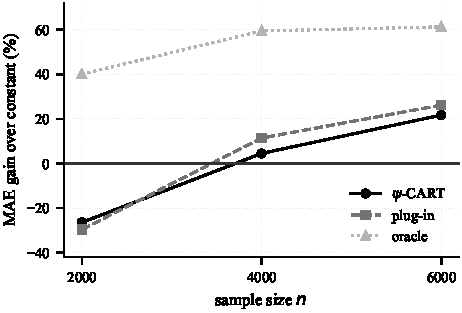
\includegraphics[width=\columnwidth]{fig1_operating_range.pdf}
\caption{Operating range of the pseudo-outcome rule model. Negative values mean
the rule model is worse than the constant. The crossover lies between 2000 and
4000 patients, and the oracle gap never closes.}
\label{fig:range}
\end{figure}

\subsection{Support-Constrained Selection}

Table~\ref{tab:support} contrasts max-mean selection with \eqref{eq:select} in
the single-region design. The support constraint triples the selected leaf
(285 to 650 patients), more than doubles the share of the true region covered
(0.228 to 0.514) and lifts ground-truth recovery from 0.216 to 0.462, at a
purity gain from 0.626 to 0.821. Commitment rises from 42.5\% to 80\% while the null-treatment rate stays
at zero and efficiency is essentially unchanged (0.847 versus 0.837).
Per-treated benefit falls slightly (0.168 to 0.162), the expected cost of
covering more patients. The pattern is the same under the two-region and
stress designs (Section~V-E), where the selectable leaf is larger and the
support constraint binds harder.

\begin{table}[t]
\caption{Single-region design: max-mean versus support-constrained selection
in CISCaRL-C200. 40 seeds, $n=8000$.}
\label{tab:support}
\centering
\footnotesize
\setlength{\tabcolsep}{3pt}
\begin{tabular}{@{}lrr@{}}
\toprule
quantity & max mean & support $\ge 200$\\
\midrule
support (patients)           & 285   & 650\\
true region covered          & 0.228 & \textbf{0.514}\\
purity                       & 0.626 & \textbf{0.821}\\
ground-truth Jaccard         & 0.216 & \textbf{0.462}\\
MAE                          & 0.0583 & 0.0587\\
commitment rate (\%)         & 42.5  & \textbf{80.0}\\
coverage                     & 0.051 & 0.142\\
per-treated effect           & 0.168 & 0.162\\
decision efficiency          & 0.847 & 0.837\\
captured benefit (committed) & 0.183 & \textbf{0.458}\\
null treatment (\%)          & 0     & 0\\
\bottomrule
\end{tabular}
\end{table}

\begin{figure}[t]
\centering
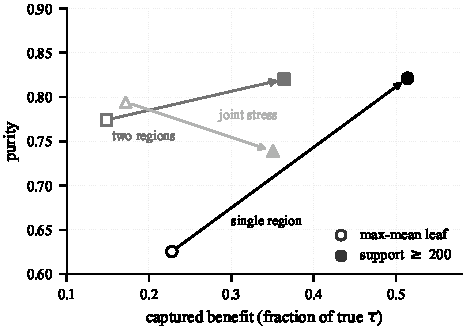
\includegraphics[width=\columnwidth]{fig2_frontier.pdf}
\caption{Capture--purity moves under the support constraint. Hollow markers are
max-mean leaves, filled markers are support-constrained leaves; arrows run from
the former to the latter. Single region gains purity and capture together; the
two-region design gains both but from a lower base; the stress design buys
capture with a purity loss of 0.055.}
\label{fig:frontier}
\end{figure}

\subsection{Stability}

Table~\ref{tab:stab} reports own-procedure refits: the whole pipeline is rerun
on disjoint discovery half-samples, and the resulting leaf is compared with the
full-data leaf. The mean Jaccard is 0.341 for C200 against 0.253 for max-mean
selection, the median rises from 0.194 to 0.297, and the share of half-samples
recovering the full-data leaf at Jaccard above 0.8 rises from 6.5\% to 9.0\%.
Raising the floor to 400 improves stability further (0.402, with 10.3\% full
recovery); in the two-region design it lowers purity to 0.778, which is the same
frontier seen from the other side. Under the non-proportional
hazards stress the C200 Jaccard falls to 0.318 with 6.6\% full recovery, so
stability is modest in absolute terms even where it improves.

\begin{table}[t]
\caption{Stability by own-procedure refits on disjoint discovery halves.
``Full'' is the share of half-samples with Jaccard $>0.8$ against the full-data
leaf; ``true'' is the Jaccard against the known region. 40 seeds.}
\label{tab:stab}
\centering
\footnotesize
\setlength{\tabcolsep}{3pt}
\begin{tabular}{@{}llrrrr@{}}
\toprule
cell & arm & mean & median & full (\%) & true\\
\midrule
$\kappa=0$ & max mean      & 0.253 & 0.194 & 6.5 & 0.348\\
$\kappa=0$ & C200          & 0.341 & 0.297 & 9.0 & 0.561\\
$\kappa=0$ & C400          & 0.402 & 0.380 & 10.3 & 0.612\\
$\kappa=3$ & C200          & 0.318 & 0.283 & 6.6 & 0.522\\
\bottomrule
\end{tabular}
\end{table}

\subsection{Two Regions and Nuisance Stress}

A single leaf cannot cover two separated regions, and
Table~\ref{tab:tworeg} quantifies the resulting ceiling. Support-constrained
selection still improves every metric with intervals excluding zero: captured
benefit 0.149 to 0.364, ground-truth recovery 0.127 to 0.295, commitment 45\%
to 70\%, and captured benefit under commitment 0.098 to 0.284. Purity rises
slightly (0.774 to 0.820) because the larger leaf is less extreme, not because
the geometry is solved. Under the joint stress the same arm raises capture from
0.172 to 0.351 and recovery from 0.148 to 0.276, but purity falls from 0.794 to
0.739, which is 0.5 percentage points beyond the pre-registered $-0.05$
tolerance. We report the miss rather than redefining the bar. The decision
layer remains safe in both designs: $0\%$ null treatment, efficiency 0.82 to
0.88, and no ATE bias ($-0.008$).

\begin{table*}[t]
\caption{Selection under two regions and under joint nuisance stress. 40 seeds,
$n=8000$, $\tau_{\text{true}}$ known analytically.}
\label{tab:tworeg}
\centering
\footnotesize
\setlength{\tabcolsep}{4pt}
\begin{tabular}{@{}llrrrrrrrr@{}}
\toprule
design & arm & support & capture & purity & J$_{\text{true}}$ & commit
(\%) & coverage & captured & null (\%)\\
\midrule
two regions & max mean      & 248 & 0.149 & 0.774 & 0.127 & 45.0 & 0.040 & 0.098 & 0\\
two regions & C200          & 678 & \textbf{0.364} & \textbf{0.820} & \textbf{0.295} & \textbf{70.0} & 0.129 & \textbf{0.284} & 0\\
\midrule
joint stress & max mean     & 290 & 0.172 & \textbf{0.794} & 0.148 & 30.0 & 0.047 & 0.115 & 0\\
joint stress & C200         & 742 & \textbf{0.351} & 0.739 & \textbf{0.276} & \textbf{57.5} & 0.148 & \textbf{0.286} & 0\\
\bottomrule
\end{tabular}
\end{table*}

\subsection{Head-to-Head with the Rule Ensemble}

Table~\ref{tab:scre} compares the model with SCRE over 80 paired replications
(two independent seed blocks) on identical splits. The frozen model is worse on
patient-level MAE: $0.0576$ versus $0.0514$ with one region
($+0.0062$, $[+0.0031,+0.0094]$, $p<0.001$) and $0.0707$ versus $0.0676$ with
two ($+0.0031$, $[+0.0001,+0.0059]$, $p=0.044$). Capture runs the other way:
SCRE captures 0.954 and 0.823 of the true effect against 0.465 and 0.277.

The accuracy loss is a calibration problem, not a selection problem. Leaf
effects estimated on 2000 validation patients are noisy, and the prediction is
a step function, so shrinking each leaf mean toward the marginal ATE
(empirical-Bayes weight from within- and between-leaf variance) lowers the mean
absolute error. Applied only to prediction, it leaves the selected rule, the
commitment decision, purity, capture and coverage unchanged to four decimals,
and it turns the comparison into a tie: $+0.0011$
$[-0.0019,+0.0042]$, $p=0.48$ with one region and $+0.0004$
$[-0.0025,+0.0033]$, $p=0.76$ with two. The shrinkage was chosen after the
original comparison and then confirmed on a fresh seed block, so we report it as
a post-hoc calibration rather than as part of the frozen design.

What remains is coverage. SCRE treats 55--56\% of assessment patients; the model
treats 13.3\% and 11.7\%. Per treated patient it delivers $0.174$ against
$0.085$ (single region) and $0.165$ against $0.101$ (two regions), and its
purity is $0.890$ and $0.858$ against $0.437$ and $0.599$. Both methods have a
zero null-treatment rate. A reader who wants the best individual-level effect
estimate should still prefer SCRE on coverage grounds; a reader who wants a
narrow, interpretable, abstention-capable policy should prefer this model, and
need no longer accept an accuracy penalty for it. Because
validation-concordance selection retains about one rule, SCRE's remaining
advantage may come from its linear predictor rather than from a usable rule
list; a multi-rule configuration is a different comparator and is not evaluated
here.

\begin{table*}[t]
\caption{Model versus SCRE on identical splits, 80 paired replications (two
seed blocks). MAE and per-treated effect use the true individual effects;
coverage is the share of assessment patients treated. C200-S is the frozen
model with empirical-Bayes shrinkage of leaf effects for prediction only;
purity, capture and coverage are identical to C200 by construction.}
\label{tab:scre}
\centering
\footnotesize
\setlength{\tabcolsep}{6pt}
\begin{tabular}{@{}llrrrrrr@{}}
\toprule
design & method & MAE & capture & purity & per-treated & coverage &
MAE vs SCRE [95\% CI]\\
\midrule
single region & C200 & 0.0576 & 0.465 & \textbf{0.890} & \textbf{+0.174} &
0.133 & $+0.0062$ [$+0.0031,+0.0094$]\\
single region & C200-S & 0.0525 & 0.465 & \textbf{0.890} & \textbf{+0.174} &
0.133 & $+0.0011$ [$-0.0019,+0.0042$]\\
single region & SCRE & \textbf{0.0514} & \textbf{0.954} & 0.437 & +0.085 &
0.548 & --\\
\midrule
two regions & C200 & 0.0707 & 0.277 & \textbf{0.858} & \textbf{+0.165} &
0.117 & $+0.0031$ [$+0.0001,+0.0059$]\\
two regions & C200-S & 0.0680 & 0.277 & \textbf{0.858} & \textbf{+0.165} &
0.117 & $+0.0004$ [$-0.0025,+0.0033$]\\
two regions & SCRE & \textbf{0.0676} & \textbf{0.823} & 0.599 & +0.101 &
0.563 & --\\
\bottomrule
\end{tabular}
\end{table*}

\subsection{Knob Sweep and Small-Sample Floor}

Before adopting the shrinkage we ran a pre-registered sweep of every remaining
knob on 40 tuning seeds, then repeated the survivors on 40 fresh seeds
(Table~\ref{tab:sweep}). Only two changes did anything. Shrinkage reduced MAE by
$0.0051$ ($p<0.001$) with one region and $0.0026$ ($p=0.014$) with two, pooled
over the 80 replications. Raising \texttt{min\_samples\_leaf} to 100 helped
slightly with two regions ($-0.0016$, $p<0.001$) and not at all with one, so it
was not adopted. Depth four was decisively worse ($+0.0099$ and $+0.0083$):
a deeper tree fits the pseudo-outcome better but selects narrower leaves, and
capture falls from 0.465 to 0.351. The commitment threshold is a policy dial,
not an accuracy lever: $z=1.28$ raises commitment from 72.5\% to 82.5\% and
lowers purity, $z=1.96$ cuts commitment to 60--70\% and raises purity, and MAE
barely moves.

\begin{table}[t]
\caption{Knob sweep, pooled over the 40 tuning and 40 confirmation seeds. Values
are paired differences in MAE against the frozen configuration (negative is
better), with 95\% bootstrap intervals.}
\label{tab:sweep}
\centering
\footnotesize
\setlength{\tabcolsep}{3pt}
\begin{tabular}{@{}lrr@{}}
\toprule
change & one region & two regions\\
\midrule
shrink leaf effects & $\mathbf{-0.0051}$ & $\mathbf{-0.0026}$\\
  & $[-0.0077,-0.0025]$ & $[-0.0048,-0.0005]$\\
\texttt{min\_leaf} 100 & $+0.0002$ & $\mathbf{-0.0016}$\\
  & $[-0.0011,+0.0015]$ & $[-0.0026,-0.0006]$\\
\texttt{min\_leaf} 30 & $-0.0002$ & $+0.0003$\\
  & $[-0.0014,+0.0011]$ & $[-0.0008,+0.0013]$\\
depth 4 & $+0.0099$ & $+0.0083$\\
  & $[+0.0080,+0.0117]$ & $[+0.0067,+0.0100]$\\
$z=1.28$ & $-0.0001$ & $-0.0001$\\
  & $[-0.0004,+0.0000]$ & $[-0.0004,+0.0000]$\\
$z=1.96$ & $+0.0005$ & $+0.0004$\\
  & $[+0.0001,+0.0010]$ & $[+0.0000,+0.0008]$\\
\bottomrule
\end{tabular}
\end{table}

The support floor is absolute (200 patients), which makes it mean different
things at different sample sizes. A separate grid compares it with a floor of
5\% of discovery. At $n=2000$ the absolute floor is 20\% of discovery and
behaves badly (purity 0.47, capture 0.096, commitment 17.5\%); the proportional
floor reaches purity 0.73, capture 0.127 and commitment 30.0\%. At $n=4000$ the
two differ only in the usual capture--purity trade (purity 0.71 versus 0.80,
capture 0.311 versus 0.281), and at $n=1000$ neither commits often because the
validation partition is too small. A proportional floor is therefore the right
specification for small samples; it is not retro-fitted to the frozen model.

\subsection{Negative Results}

Table~\ref{tab:neg} lists the rejected alternatives. The two-leaf list captures
more of the two-region truth (0.414 to 0.584) but dilutes purity from 0.862 to
0.696 and fails the purity bar. The flexible doubly robust learner with
distillation produces a purer (0.897) but narrower rule and loses capture
(0.548 to 0.454; $-0.07$ to $-0.09$ across designs); its distillation minimum
(200 versus C200's 60) makes the comparison conservative, so the negative
applies to the tested implementation, not to flexible learning in general. The
plug-in target collapses under $\kappa=3$, confirming that a target defined by
dividing by an estimated density is not robust to nuisance misspecification.
These are points on the capture--purity frontier, not a sequence of failed
attempts to find a dominant method.

\begin{table}[t]
\caption{Documented negative results.}
\label{tab:neg}
\centering
\footnotesize
\setlength{\tabcolsep}{3pt}
\begin{tabular}{@{}p{0.29\columnwidth}p{0.07\columnwidth}p{0.56\columnwidth}@{}}
\toprule
lever & exp. & outcome\\
\midrule
RMST & 8 & signal-to-noise 0.20$\to$0.19; worse than constant\\
min support & 7 & no gain through the previous target\\
RF + stability & 9--12 & too few rules at small $n$\\
plug-in, $\kappa=3$ & 14 & collapses; $\psi$ survives\\
target blend & 15 & does not rescue; $\psi$ alone is better\\
two-leaf list & 25 & capture $+0.169$, purity $-0.166$; rejected\\
flexible learner & 26 & capture $-0.07$ to $-0.09$, purity $+0.06$; rejected\\
\bottomrule
\end{tabular}
\end{table}

\section{Application to ACTG175}

ACTG175 is a randomized HIV trial comparing nucleoside regimens
\cite{actg,actgdata}. We use arms 0 and 1 (AZT versus AZT plus ddI), giving
$n=1054$ patients and 12 baseline covariates (\texttt{cd40}, \texttt{cd80},
\texttt{age}, \texttt{wtkg}, \texttt{karnof}, \texttt{hemo}, \texttt{homo},
\texttt{race}, \texttt{gender}, \texttt{drugs}, \texttt{str2},
\texttt{symptom}), with no missing values in these columns. The endpoint is the
composite progression-free event defined in Section~III, and the horizon is 730
days. Preprocessing follows the honest rule: the cohort is split first
(527 discovery, 263 validation, 264 assessment), the standardization is fitted
on discovery only and applied unchanged to validation and assessment.

The overall assessment contrast is $\tau(730)=+0.143$ with $95\%$ interval
$[+0.025,+0.262]$, a \textsc{treat} verdict for the average patient. The
support constraint, however, is not achievable at this sample size: the largest
discovered leaf contains 174 patients, below the floor of 200, so the procedure
falls back to the max-mean leaf
\texttt{cd40}${}\le343.5$ \& \texttt{age}${}>28.5$ \& \texttt{homo}${}\le0.5$
with 62 discovery patients. Its validation effect is $+0.085$ (SE $0.189$), so
the one-sided lower bound is $-0.226$ and the model does not commit; the
decision is \textsc{insufficient}. The assessment estimate for the leaf is
$+0.540$ $[+0.178,+0.901]$ on 30 patients, and the censoring-weight tilt moves
it between $+0.447$ and $+0.623$ (Fig.~\ref{fig:tilt}). Both the point estimate
and the interval rest on 30 patients; they are descriptive, not a subgroup
recommendation.

This is the intended behaviour at the sample-size boundary: the support rule
cannot bind, the fallback leaf is small, and the commitment layer abstains
instead of reporting a winner's-curse effect. The real data contain no known
treatment-effect truth, so capture, purity, MAE and Jaccard are not computable
here; they appear only in the simulation study.

Table~\ref{tab:rules} lists every candidate rule from the discovery tree in the
format used for rule-ensemble output. Three columns are translated rather than
copied. Ensemble \emph{importance} becomes the discovery mean pseudo-outcome
$\bar\psi$ together with a relative score $100\,\bar\psi/\max\bar\psi$,
because a tree has no coefficient to normalize. \emph{Support} is the quantity
the model actually constrains, so it is reported with its share of the
discovery partition. The hazard ratio is added only for comparability: it is a
treated-versus-control Cox fit inside each leaf on the assessment partition, it
is not the estimand, and it rests on 30--91 patients. The paper's claims rest
on the 730-day contrast, not on these ratios.

The number of rows differs by construction. A depth-3 tree yields five leaves
here and the frozen policy commits to at most one, so there is no sixteen-rule
list to report; the sixteen-rule output of a rule ensemble comes from a
different model class and a different regularization path. Two features of the
table are worth noting. The selected leaf has both the largest discovery score
(0.478) and the largest assessment contrast (0.540), yet its validation
contrast is only 0.085, which is exactly why the model abstains. And leaf~3 has
the second-largest discovery score but a negative assessment contrast
($-0.297$), so a depth-3 partition can separate groups whose effects do not
replicate: the score ranks candidates, it does not certify them.

Table~\ref{tab:km} adds the check that rule-ensemble papers usually report on
real data: for each candidate rule, the unadjusted Kaplan--Meier survival at 730
days in each arm and the observed difference, with a bootstrap interval
\cite{scre}. This is descriptive and optimistic, because the rules were
selected on the discovery partition and the curves use every patient; it can
confirm direction, not accuracy. Three readings follow. The marginal difference
is $+0.133$ $[+0.084,+0.179]$, close to the AIPW overall estimate of $+0.143$,
which supports the estimation pipeline. The selected leaf has the largest
observed difference of the five ($+0.322$ $[+0.171,+0.468]$), consistent with
its AIPW assessment value. Leaf~3 does not follow its AIPW point estimate: the
$\hat\tau=-0.297$ obtained on 30 assessment patients is not reproduced by the
unadjusted curves ($+0.081$ $[-0.021,+0.183]$), so the negative value should not
be read as evidence of harm — it is what a 30-patient influence-function
estimate looks like under noise, and it is one more reason the model does not
commit on this sample.

\begin{table*}[t]
\caption{All candidate rules from the ACTG175 discovery tree. $\bar\psi$ is
the discovery mean AIPW pseudo-outcome with its standard error; rel.\ is
$100\,\bar\psi/\max\bar\psi$; support is discovery patients and the share of
the discovery partition; the $\hat\tau$ columns are AIPW estimates with 95\%
confidence intervals on the validation and assessment partitions; HR is a
descriptive treated-versus-control hazard ratio inside the leaf on assessment,
reported for comparability with rule-ensemble output and not the estimand.
$\star$ marks the leaf the frozen policy selects.}
\label{tab:rules}
\centering
\scriptsize
\setlength{\tabcolsep}{3pt}
\begin{tabular}{@{}r p{0.245\textwidth} rrrrrr@{}}
\toprule
\# & rule & $\bar\psi$ (SE) & rel. & support (\%) & val.\ $\hat\tau$ [CI]
& asm.\ $\hat\tau$ [CI] & HR [CI]\\
\midrule
1 & \texttt{age} $\le$ 28.5 & $-0.010$ (0.101) & $-2$ & 114 (21.6)
& 0.331 [0.046, 0.616] & 0.171 [$-$0.093, 0.434] & 0.39 [0.13, 1.14]\\
2$^{\star}$ & \texttt{cd40} $\le$ 343.5 \& \texttt{age} $>$ 28.5 \&
\texttt{homo} $\le$ 0.5 & \textbf{0.478} (0.113) & \textbf{100} &
\textbf{62 (11.8)} & \textbf{0.085} [$-$0.299, 0.468] &
\textbf{0.540} [0.178, 0.901] & \textbf{0.10} [0.02, 0.52]\\
3 & \texttt{cd40} $>$ 343.5 \& \texttt{age} $>$ 28.5 \& \texttt{homo} $\le$ 0.5
& 0.244 (0.123) & 51 & 62 (11.8) & 0.324 [0.025, 0.622] &
$-0.297$ [$-$0.619, 0.024] & 1.50 [0.34, 6.74]\\
4 & \texttt{cd80} $\le$ 1093.5 \& \texttt{age} $>$ 28.5 \& \texttt{homo} $>$ 0.5
& 0.035 (0.074) & 7 & 174 (33.0) & 0.141 [$-$0.068, 0.349] &
0.090 [$-$0.104, 0.283] & 0.56 [0.24, 1.32]\\
5 & \texttt{cd80} $>$ 1093.5 \& \texttt{age} $>$ 28.5 \& \texttt{homo} $>$ 0.5
& 0.299 (0.089) & 63 & 115 (21.8) & 0.090 [$-$0.165, 0.346] &
0.227 [$-$0.039, 0.494] & 0.43 [0.18, 1.03]\\
\midrule
& marginal ATE & 0.160 & -- & 527 (100) & -- & 0.143 [0.025, 0.262] & --\\
\bottomrule
\end{tabular}
\end{table*}

\begin{table}[t]
\caption{Unadjusted Kaplan--Meier check of every candidate rule on ACTG175 (all
$n=1054$ patients). $S_{1}$ and $S_{0}$ are survival at 730 days in the treated
and control arms; $\Delta S$ is their difference with a bootstrap 95\% interval;
$\bar\psi$ is the discovery score from Table~\ref{tab:rules}. The check
confirms direction only: the rules were selected on discovery and these curves
reuse every patient, so the comparison is optimistic.}
\label{tab:km}
\centering
\scriptsize
\setlength{\tabcolsep}{2pt}
\begin{tabular}{@{}r p{0.26\columnwidth} r r r r r@{}}
\toprule
\# & rule & $n$ & $S_{1}$ & $S_{0}$ & $\Delta S$ [95\% CI] & $\bar\psi$\\
\midrule
1 & \texttt{age} $\le$ 28.5 & 226 & 0.824 & 0.747 & 0.077 [$-$0.039, 0.199] & $-0.010$\\
2$^{\star}$ & \texttt{cd40} $\le$ 343.5 \& \texttt{age} $>$ 28.5 \&
\texttt{homo} $\le$ 0.5 & 128 & 0.921 & 0.599 &
\textbf{0.322} [0.171, 0.468] & \textbf{0.478}\\
3 & \texttt{cd40} $>$ 343.5 \& \texttt{age} $>$ 28.5 \& \texttt{homo} $\le$ 0.5
& 127 & 0.945 & 0.865 & 0.081 [$-$0.021, 0.183] & 0.244\\
4 & \texttt{cd80} $\le$ 1093.5 \& \texttt{age} $>$ 28.5 \& \texttt{homo} $>$ 0.5
& 350 & 0.855 & 0.766 & 0.089 [0.012, 0.172] & 0.035\\
5 & \texttt{cd80} $>$ 1093.5 \& \texttt{age} $>$ 28.5 \& \texttt{homo} $>$ 0.5
& 223 & 0.848 & 0.644 & 0.204 [0.101, 0.313] & 0.299\\
\midrule
& all patients & 1054 & 0.865 & 0.732 & 0.133 [0.084, 0.179] & --\\
\bottomrule
\end{tabular}
\end{table}

\begin{figure}[t]
\centering
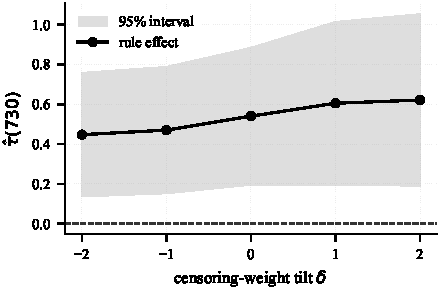
\includegraphics[width=0.92\columnwidth]{fig3_actg175_tilt.pdf}
\caption{ACTG175 sensitivity of the fallback leaf's assessment effect to a
censoring-weight tilt $\delta\in[-2,2]$. The effect stays positive, but every
interval is wide and the model has already declined to commit.}
\label{fig:tilt}
\end{figure}

\section{Discussion and Limitations}

The empirical finding is a boundary, not a victory. At small samples the rule
model is worse than the constant; at $n\ge6000$ it beats the constant; and the
size of the gain depends on the truth structure. The constant baseline is what
makes this visible: without it, a method that predicts the marginal effect for
everyone can look like a success.

The support constraint addresses a real selection problem. It raises capture,
ground-truth recovery and reproducibility across a single-region and a
two-region design, and it improves the stability of the selected leaf. It does
not recover multiple regions: one leaf captures 33--59\% of the true benefit,
depending on the designs compared. A two-leaf list captures more but dilutes
purity; a flexible learner produces a purer but narrower rule. These are points
on a frontier, and the paper's contribution is to locate them, not to claim a
dominant method.

Validation-based commitment is the most robust component. It converts an
uncertain high-effect leaf into an abstention: zero null-benefit treatment in
the tested cells, decision efficiency 0.82--0.88, at a coverage cost. On
ACTG175 it abstains exactly where a naive analysis would have reported a large
subgroup effect.

The comparison with SCRE sharpens the claim. On patient-level accuracy the
ensemble wins against the frozen model and ties with the shrunk one; on subgroup
purity and per-treated benefit the rule model wins by a factor of two. Reporting
only one of the two would misrepresent the trade in the opposite direction. The
shrinkage result also illustrates why calibration and selection must be
separated: the same rule, with the same commitment decisions, moved from a
significant accuracy deficit to a tie purely by treating noisy leaf means as
noisy.

Several limitations bound these conclusions. The shrinkage that removes the
accuracy deficit was chosen after the original SCRE comparison, so it is a
post-hoc calibration confirmed on a fresh seed block, not part of the frozen
pre-registered design; the frozen configuration remains the one in Tables
I--IV. Capture is 0.33--0.59, so the
selected leaf is a high-purity subset rather than the true region. Stability is
modest in absolute terms: mean Jaccard 0.34, and fewer than one half-sample in
ten recovers the full-data leaf at Jaccard above 0.8. The joint stress cell
misses the purity tolerance by 0.5 percentage points. The main design uses one
partition ratio (4000/2000/2000) at one sample size, and the gain is sensitive
to that choice; the operating-range table reports the ratio actually used at
each $n$ rather than smoothing across designs. Two mechanisms are studied, both
built on the ACTG175 covariate matrix, so nothing is claimed beyond that
family. The estimand is fixed-time only; restricted mean survival and
hazard-ratio estimands are separate decisions, and the restricted-mean variant
performed worse than its own constant in our tests. Intervals are
influence-function based, conditional on the selected rule, and cover
approximately $93\%$, not $95\%$; selection-aware inference for the committed
rule effect is not implemented. The SCRE comparison covers one regularization
path that retains about one rule, so its multi-rule behaviour is untested here.
Finally, ACTG175 is an illustration: the true subgroup is unknown, the endpoint
is composite, and the observed follow-up process limits any causal reading.

\section{Conclusion}

Support-constrained selection plus validation-based commitment yields an
interpretable survival subgroup model (CISCaRL, configuration C200) with a
measured operating range: unusable
at 2000 patients, reliable from roughly 6000, and worth about a fifth of the
constant model's error at 8000. The support floor is what converts an
optimistic best leaf into a policy that captures more of the true benefit at
higher purity, and the commitment layer is what prevents a small fallback leaf
from being reported as a finding. Against a survival rule ensemble on identical
splits the frozen model is slightly less accurate per patient; after shrinking
the leaf effects for prediction only, the two are statistically tied on
patient-level error, while the rule model is much purer, roughly twice as
beneficial per treated patient, and capable of abstaining. The contribution is
therefore precision, calibration and abstention - not coverage, and not raw
predictive dominance.
Future work should test external validation, a diagonal rule geometry, and
selection-aware inference for the committed rule effect, whose current
intervals are conditional on the selected rule and cover approximately $93\%$,
not $95\%$.

\section*{Reproducibility}

All simulation cells are pre-registered under \texttt{results/} with their
verdicts, and the replications use non-overlapping seeds. The rule
implementation and its audit are in \texttt{ciscarl2/rules.py} and
\texttt{ciscarl2/audit.py}. The complete pipeline, from raw ACTG175 to every
number reported here, is a single executed notebook
(\texttt{notebooks/CISCaRL\_final.ipynb}); fragmentation of results across
scripts is not required to reproduce the paper.

\begin{thebibliography}{00}
\bibitem{bang} H.~Bang and J.~M.~Robins, ``Doubly robust estimation in missing
data and causal inference models,'' \emph{Biometrics}, vol.~61, no.~4,
pp.~962--973, 2005.

\bibitem{dml} V.~Chernozhukov, D.~Chetverikov, M.~Demirer, E.~Duflo,
C.~Hansen, W.~Newey, and J.~Robins, ``Double/debiased machine learning for
treatment and structural parameters,'' \emph{The Econometrics Journal},
vol.~21, no.~1, pp.~C1--C68, 2018.

\bibitem{drlearner} E.~M.~Athey and S.~Wager, ``Estimating treatment effects
with causal forests: an application,'' \emph{Observational Studies}, vol.~5,
pp.~37--51, 2019.

\bibitem{nie} X.~Nie and S.~Wager, ``Quasi-oracle estimation of heterogeneous
treatment effects,'' \emph{Biometrika}, vol.~108, no.~2, pp.~299--319, 2021.

\bibitem{kunzel} S.~R.~K\"unzel, J.~S.~Sekhon, P.~J.~Bickel, and B.~Yu,
``Metalearners for estimating heterogeneous treatment effects using machine
learning,'' \emph{Proceedings of the National Academy of Sciences}, vol.~116,
no.~10, pp.~4156--4165, 2019.

\bibitem{csf} Y.~Cui, M.~R.~Kosorok, E.~Sverdrup, S.~Wager, and R.~Zhu,
``Causal survival forests,'' \emph{arXiv preprint arXiv:2304.10577}, 2023.

\bibitem{wager} S.~Wager and S.~Athey, ``Estimation and inference of
heterogeneous treatment effects using random forests,'' \emph{Journal of the
American Statistical Association}, vol.~113, no.~523, pp.~1228--1242, 2018.

\bibitem{foster} J.~C.~Foster, J.~M.~G.~Taylor, and S.~J.~Ruberg, ``Subgroup
identification from randomized clinical trial data,'' \emph{Statistics in
Medicine}, vol.~30, no.~24, pp.~2867--2880, 2011.

\bibitem{lipkovich} I.~Lipkovich, A.~Dmitrienko, and R.~B.~D'Agostino~Sr.,
``Tutorial in biostatistics: data-driven subgroup identification and analysis
in clinical trials,'' \emph{Statistics in Medicine}, vol.~36, no.~1,
pp.~136--196, 2017.

\bibitem{rulefit} J.~H.~Friedman and B.~E.~Popescu, ``Predictive learning via
rule ensembles,'' \emph{Annals of Applied Statistics}, vol.~2, no.~3,
pp.~916--954, 2008.

\bibitem{scre} K.~Wan, K.~Tanioka, and T.~Shimokawa, ``Survival causal rule
ensemble method considering the main effect for estimating heterogeneous
treatment effects,'' preprint, 2025.

\bibitem{stability} N.~Meinshausen and P.~B\"uhlmann, ``Stability selection,''
\emph{Journal of the Royal Statistical Society: Series B}, vol.~72, no.~4,
pp.~417--473, 2010.

\bibitem{policy} S.~Athey and S.~Wager, ``Policy learning with observational
data,'' \emph{Econometrica}, vol.~89, no.~1, pp.~133--161, 2021.

\bibitem{actg} S.~M.~Hammer \emph{et al.}, ``A trial comparing nucleoside
monotherapy with combination therapy in HIV-infected adults with CD4 cell
counts from 200 to 500 per cubic millimeter,'' \emph{New England Journal of
Medicine}, vol.~335, no.~15, pp.~1081--1090, 1996.

\bibitem{actgdata} J.~Juraska and P.~B.~Gilbert, ``\emph{speff2trial}:
Semiparametric efficient estimation for a two-sample treatment effect,'' R
package, CRAN.

\end{thebibliography}

\end{document}
